\documentclass{beamer}
\usetheme{Pittsburgh}
\beamertemplatenavigationsymbolsempty


\usepackage{amsmath}
\usepackage{amssymb}
\usepackage{bm} % For bold math symbols
\usepackage{graphicx}
\usepackage{tikz}



\usepackage{subfig} % Changed from subfigure (deprecated)
\usepackage{multirow}
\usepackage{multicol}
\usepackage{color}
\usepackage{url}
\usepackage{hyperref}
\usepackage{listings}
\usepackage[noend]{algorithm}
\usepackage{physics} 
% add image path
\graphicspath{{../Images/}}






\DeclareMathOperator{\argmin}{argmin}
\DeclareMathOperator{\argmax}{argmax}






\title{Weekly Updates\\
\tiny{Wednesday, 12/03/2025}}
\author{Andrea Bonifacio}
\date{}

\begin{document}

\begin{frame}
\titlepage
\end{frame}

\begin{frame}{Recap: Project Goals \& Status}
    \begin{itemize}
        \item Here's a brief recap of what we did up until now.
        \item In the first half of this project we started implementing a method that uses neural networks to compute the nonlinear correction of the displacement field.
        \item The idea was interesting, with some already existing methods in the field of CFD, but at some point we realized that the method was not easily applicable to our case, especially for the dynamic case.
        \item We decided to explore a different method, which is based on the idea of using a neural network to ``correct'' the linear modes of a structure.
    \end{itemize}
\end{frame}

\begin{frame}{Overview of Work Done}
    \begin{itemize}
        \item While the first part of the project was not very successful, helped us a lot to understand the problem and create the necessary tools to implement the new method.
        \item We learned the limitations and strengths of the numerical solver we are using (SOFA).
        \item The main idea is still to somehow correct a displacement field, but this new method is based on a self-supervised approach, removing the need for a dataset.
    \end{itemize}
\end{frame}


\begin{frame}{New Approach: Enhanced Reduced Order Models}
    \begin{itemize}
        \item \textbf{Main Goal:} Study the efficacy of a Reduced Order Model (ROM) based on linear modes, enhanced by Deep Learning.
        \item \textbf{Objective:} Achieve realistic simulations significantly faster than traditional FEM.
        \item \textbf{Core Idea:} Train a DL model to correct linear modes.
    \end{itemize}
\end{frame}

\begin{frame}{Mathematical Framework Overview}
    \begin{itemize}
        \item Our approach integrates three core elements:
        \begin{enumerate}
            \item \textbf{Hyperelastic Mechanical Model:} Represents material's constitutive behavior.
            \item \textbf{Linear Modal Analysis:} For efficient dimensionality reduction.
            \item \textbf{Neural Modes Technique:} Incorporates nonlinear effects.
        \end{enumerate}
        \item \textbf{Goal:} Accurate and computationally tractable simulations of soft tissue deformation.
    \end{itemize}
\end{frame}

\begin{frame}{Mechanical Model: Kinematics}
    \begin{itemize}
        \item \textbf{Reference Configuration:} Material coordinates \(\bm{X}\).
        \item \textbf{Deformation:} Displacement vector \(\bm{u}(\bm{X},t)\).
        \item \textbf{Deformed Configuration:} Spatial coordinates \(\bm{x}(\bm{X},t)\).
        \begin{equation*}
            \bm{x}(\bm{X},t) = \bm{X} + \bm{u}(\bm{X},t)
        \end{equation*}
        \item Focus on hyperelastic models for soft tissues (e.g., Neo-Hookean) to handle large, nonlinear deformations.
    \end{itemize}
\end{frame}

\begin{frame}{Mechanical Model: Neo-Hookean Hyperelasticity}
    \begin{itemize}
        \item \textbf{Deformation Gradient:}
        \begin{equation*}
            \bm{F} = \frac{\partial \bm{x}}{\partial \bm{X}} = \bm{I} + \nabla_X \bm{u}
        \end{equation*}
        \item \textbf{Neo-Hookean Strain-Energy Density Function \(\Psi\):}
        \begin{equation*}
            \Psi(\bm{F}) = \frac{\mu}{2} (I_C - 3 - 2\ln(J)) + \frac{\lambda}{4} (J^2 - 1 - 2\ln(J))
        \end{equation*}
        \item \(J = \det(\bm{F})\), \(\mu\) (shear modulus), \(\lambda\) (Lamé's first parameter).
        \item Material parameters related to Young's modulus \(E\) and Poisson's ratio \(\nu\).
    \end{itemize}
\end{frame}


\begin{frame}{Linear Modal Analysis: Motivation}
    \begin{itemize}
        \item Simulating deformations in real-time is computationally challenging.
        \item \textbf{Modal Analysis:} Accelerates simulations by approximating complex deformations as a combination of dominant vibration patterns (modes).
        \item Reduces dimensionality by focusing on low-frequency modes.
        \item Enables faster simulations while maintaining reasonable accuracy for certain regimes.
    \end{itemize}
\end{frame}

\begin{frame}{Linear Modal Analysis: Core Steps}
    \begin{enumerate}
        \item \textbf{Linearize the System:}
        \begin{itemize}
            \item Linearize governing equations around undeformed state (\(\bm{u}=\bm{0}\)).
            \item Results in constant stiffness matrix \(\bm{K}\) and mass matrix \(\bm{M}\).
        \end{itemize}
        \item \textbf{Solve Generalized Eigenvalue Problem:}
        \begin{equation*}
            \bm{K} \bm{\phi}_i = \omega_i^2 \bm{M} \bm{\phi}_i
        \end{equation*}
        \begin{itemize}
            \item \(\omega_i^2\): Eigenvalues (squared natural frequencies).
            \item \(\bm{\phi}_i\): Eigenvectors (mode shapes).
        \end{itemize}
    \end{enumerate}
\end{frame}

\begin{frame}{Linear Modal Analysis: Modal Decomposition \& Limitations}
    \begin{itemize}
        \item \textbf{Modal Decomposition (Reduced Basis):}
        \begin{itemize}
            \item Select first \(m\) modes (lowest frequencies).
            \item Approximate displacement:
            \begin{equation*}
                \bm{u}(\bm{X},t) \approx \sum_{i=1}^{m} q_i(t) \bm{\phi}_i(\bm{X})
            \end{equation*}
            \item \(q_i(t)\): Time-varying modal coordinates.
        \end{itemize}
        \item \textbf{Fundamental Limitation:}
        \begin{itemize}
            \item Initial linearization holds well only for \textbf{small deformations}.
            \item Breaks down for large, nonlinear deformations (e.g., hyperelastic materials).
            \item Constant \(\bm{K}\) doesn't capture nonlinear material resistance.
        \end{itemize}
        \item \textbf{Motivation for Neural Modes:} Overcome these limitations by incorporating nonlinear effects.
    \end{itemize}
\end{frame}


\begin{frame}{Neural Modes Architecture}
    \begin{itemize}
        \item \textbf{Goal:} Learn nonlinear corrections to linear deformation modes for Neo-Hookean materials.
        \item \textbf{Input:} Modal coordinate vector \( \bm{z} \in \mathbb{R}^m \).
        \item \textbf{Core:} Deep residual neural network.
        \begin{itemize}
            \item Several residual blocks (fully connected layers + Leaky ReLU + skip connection).
        \end{itemize}
        \item \textbf{Output:} Nonlinear correction to displacement field \( \bm{y} \in \mathbb{R}^n \).
        \item \textbf{Concept:} Maps low-dimensional modal space \(\bm{z}\) to high-dimensional correction \(\bm{y}\).
    \end{itemize}
    \begin{center}
    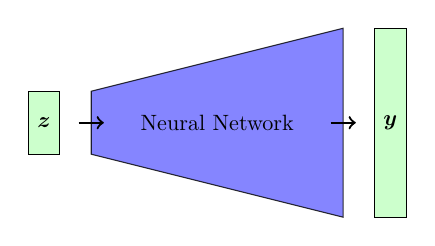
\begin{tikzpicture}[scale=0.8, transform shape]
        % Modal coordinate (z)
        \draw[fill=green!20] (-3, 1) rectangle (-2.5,2);
        \node at (-2.75, 1.5) {$\bm{z}$};
        % Neural Network
        \draw[fill=blue!60,opacity=0.8] (-2,1) -- (2,-0) -- (2,3) -- (-2,2) -- cycle;
        \node at (0,1.5) {Neural Network};
        % Displacement (y)
        \draw[fill=green!20] (2.5,0) rectangle (3,3);
        \node at (2.75, 1.5) {$\bm{y}$};
        % Arrow and Text
        \draw[thick,->] (-2.2, 1.5) -- (-1.8,1.5); % z to NN
        \draw[thick,->] (1.8,1.5) -- (2.2,1.5); % NN to y
    \end{tikzpicture}
    \end{center}
\end{frame}

\begin{frame}{Training Neural Modes: Physics-Informed Loss}
    \begin{itemize}
        \item Self-supervised: Minimize physics-based losses, not just prediction error.
        \item \textbf{Total Loss:} Weighted sum of:
        \begin{enumerate}
            \item \textbf{Energy Loss:} Minimize internal strain energy \(E(\bm{X} + \bm{l} + \bm{y})\).
            \begin{itemize}
                \item \(\bm{l}\): linear displacement from \(\bm{z}\).
                \item \(\bm{y}\): nonlinear correction from NN.
            \end{itemize}
            \item \textbf{Orthogonality Loss:} Ensure correction \(\bm{y}\) is orthogonal to linear modes: \(\bm{y}^T \bm{l} = 0\).
            \item \textbf{Boundary Condition Penalty:} Enforce displacement BCs.
        \end{enumerate}
        \begin{equation*}
            \text{Loss} = E(\bm{X} + \bm{l} + \bm{y}) + \lambda_1 (\bm{y}^T \bm{l})^2 + \lambda_2 \text{BC Penalty}
        \end{equation*}
        \item \textbf{Zero Correction at Origin:} Ensured by bias-free NN architecture (output is zero if \(\bm{z}=\bm{0}\)).
    \end{itemize}
\end{frame}

\begin{frame}{Subspace Learning: Efficiently Finding Solutions}
    \begin{itemize}
        \item \textbf{Problem:} Find displacement \(\bm{x}^*\) minimizing energy \(E_\phi(\bm{x})\) subject to constraints \(C_\psi(\bm{x})=0\).
        \begin{equation*}
            \bm{x}^*(\phi, \psi) = \underset{\bm{x}}{\argmin} E_\phi(\bm{x}) \quad \text{s.t.} \quad C_\psi(\bm{x}) = 0
        \end{equation*}
        \item Classical FEM solves this for each configuration (expensive).
        \item \textbf{Idea (Wang et al.):} Approximate \(\bm{x}^*\) with a NN \(\bm{x}[\theta^*](\phi, \psi)\).
        \item \textbf{Our Application (Neural Modes):}
        \begin{itemize}
            \item Nonlinear modes \(\bm{n}(\bm{z}) = \bm{l} + \bm{y}[\theta^*](\bm{z})\).
            \item Train NN \(\bm{y}[\theta](\bm{z})\) by minimizing the physics-informed loss:
            \begin{equation*}
                \mathcal{L}(\theta) = \mathbb{E}_{\bm{z}} \left[ E(\bm{X} + \bm{l} + \bm{y}[\theta]) + \lambda_1 (\bm{l}^T \bm{y}[\theta])^2 + \dots \right]
            \end{equation*}
        \end{itemize}
    \end{itemize}
\end{frame}

\begin{frame}{Dynamic Simulation with Neural Modes}
    \begin{itemize}
        \item At each time step \(n+1\), solve for modal coordinates \(\bm{z}_{n+1}\):
        \begin{equation*}
            \bm{z}_{n+1} = \underset{\bm{z}}{\argmin} \frac{1}{2h^2} \|\bm{n}(\bm{z}) - 2\bm{u}_n + \bm{u}_{n-1}\|_{\bm{M}}^2 + E(\bm{n}(\bm{z}))
        \end{equation*}
        \begin{itemize}
            \item \(\bm{n}(\bm{z}) = \bm{l}(\bm{z}) + \bm{y}(\bm{z})\): Full displacement (linear + NN correction).
            \item \(h\): time step, \(\bm{M}\): mass matrix.
            \item Solved using L-BFGS-B.
        \end{itemize}
        \item \textbf{Challenge:} Current formulation doesn't explicitly account for external forces.
        \begin{itemize}
            \item Network minimizes internal energy.
            \item May affect accuracy for large deformations or complex external loads.
        \end{itemize}
    \end{itemize}
\end{frame}




\begin{frame}{Neural Modes Paper - Key Ideas}
    \begin{itemize}
        \item The paper wants to extend the concept of linear modes to ``neural modes''.
        \item The idea is to compute a non-linear correction of the displacement field, by having the network minimize the energy of the system.
        \item Once the network has been trained and learned the non-linear modes for any modal coordinate in the subspace, it can be extended to dynamics by using a finite difference scheme.
    \end{itemize}
\end{frame}



\begin{frame}{Neural Modes Paper - Our Implementation}
    \begin{itemize}
        \item We developed a fully differentiable energy calculator for both StVenant-Kirchhoff and Neo-Hookean materials, completely written in PyTorch, that helps with the training speed.
        \item Most of the deformation is already captured by the linear modes (the nonlinear correction is small, around 1\%).
        \item I am having problem with changing the material properties during the simulation.
    \end{itemize}
\end{frame}




\begin{frame}{Neural Modes Paper - Critical Review}
    \begin{itemize}
        \item After implementing both StVenant-Kirchhoff and Neo-Hookean materials, I realized that this method works well for small deformations.
        \item Most of the deformation is already captured by the linear modes (the nonlinear correction is small, around 1\%).
        \item I am having problem with changing the material properties during the simulation.
    \end{itemize}
\end{frame}


\begin{frame}
    \frametitle{Network Architecture}
    \begin{itemize}
        \item The network is a feedforward neural network.
        \item The input is the modal coordinate \( z \in \mathbb{R}^m \).
        \item The output is a correction on the displacement field \( \mathbf{y} \in \mathbb{R}^n \).
    \end{itemize}



\begin{center}
        
        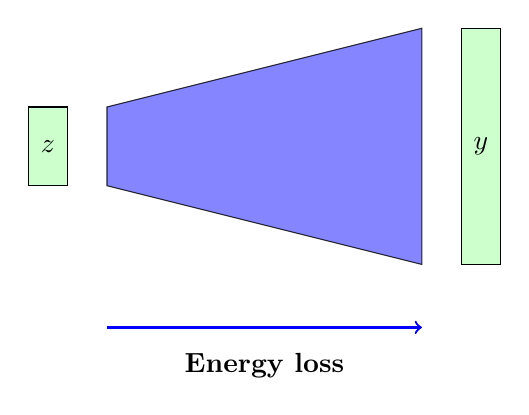
\begin{tikzpicture}
            % Modal coordinate (z)
            \draw[fill=green!20] (-3, 1) rectangle (-2.5,2);
            \node at (-2.75, 1.5) {$z$}; % Label inside the rectangle
            
            % Displacement (u)
            \draw[fill=green!20] (2.5,0) rectangle (3,3);
            \node at (2.75, 1.5) {$y$}; % Label inside the rectangle
            
            % Energy loss transition
            \draw[fill=blue!60,opacity=0.8] (-2,1) -- (2,-0) -- (2,3) -- (-2,2) -- cycle;
            \node[below] at (0,-1) {\textbf{Energy loss}};
            
            % Energy loss arrow
            \draw[thick,blue,->] (-2,-0.8) -- (2,-0.8);
        
        \end{tikzpicture}
\end{center}
    
\end{frame}

\begin{frame}
    \frametitle{Training the network}
    \begin{itemize}
        \item At each iteration, the network is trained on a batch of modal coordinates randomly selected.
        \item Four loss functions are used:
        \begin{itemize}
            \item Energy loss: \( E(X + l + y)\), where \(X\) is the rest position, \(l\) is the linear mode given by \(z\) and \(y\) is the nonlinear correction.
            \item Orthogonality loss: \( y^T l = 0 \).
            \item Origin loss: \( y(0) = 0 \).
        \end{itemize}
        \item The network is trained by minimizing the weighted sum of these losses.
        \[
        \text{Loss} = \text{Energy } + \lambda_1 \text{Orthogonality } + \lambda_2 \text{Origin}
        \]
    \end{itemize}
\end{frame}

\begin{frame}
    \frametitle{Visualization}
    \begin{figure}
        \centering
        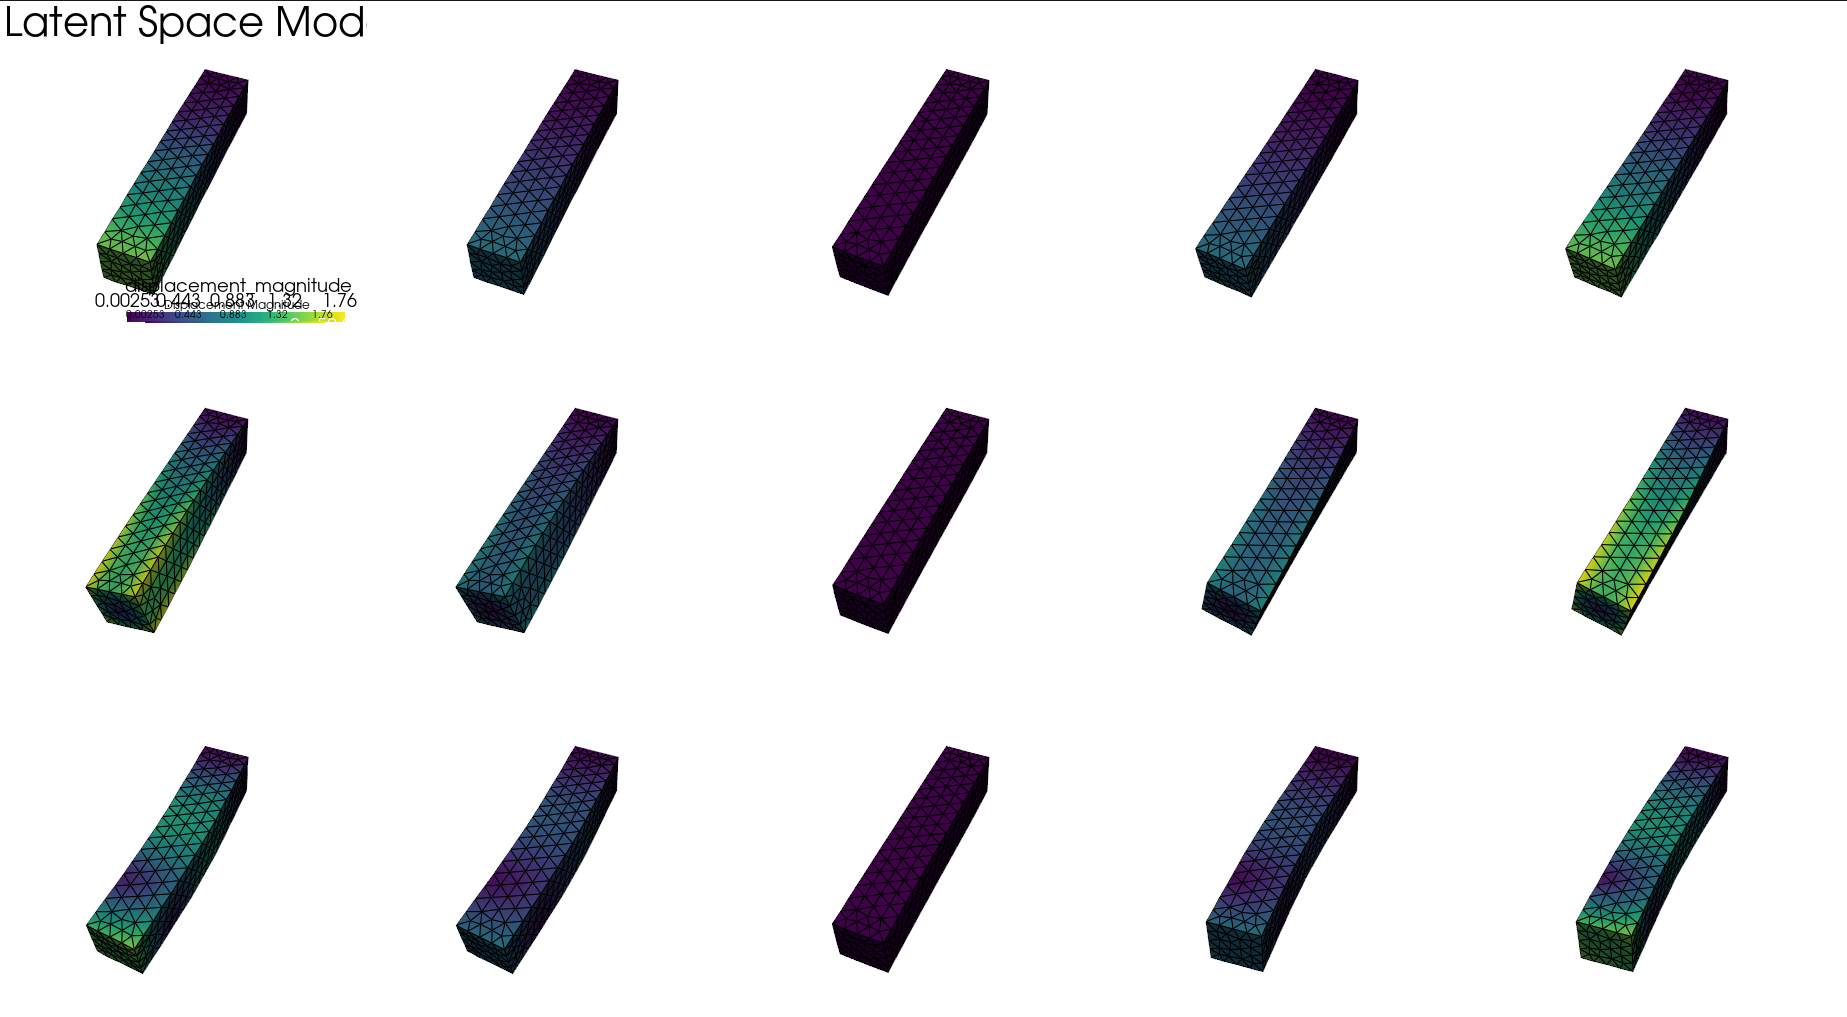
\includegraphics[scale=0.15]{Images/image.png}
        \caption{Nonlinear latent space.}
    \end{figure}
\end{frame}

\begin{frame}
    \frametitle{Dynamic simulation}
    I started implementing it, but the optimization problem takes too long to solve.
    \begin{itemize}
        \item The optimization problem is solved using the L-BFGS-B algorithm. (As in the paper)
        \item Each iteration takes around 3-4 seconds.
        \item Maybe another optimization algorithm could be used?
    \end{itemize}
    \begin{itemize}
        \item The non-linear correction can be computed by:
        \[
        z_{n+1} = \underset{z}{\argmin}  \frac{1}{2h^2} \norm{n(z) - 2u_n + u_{n-1}}^2_M + E(n(z))
        \]
        \item Here \(n(z)\) is the non-linear correction computed by the network, and \(M\) is the mass matrix.
    \end{itemize}
\end{frame}

\begin{frame}
    \frametitle{What now?}
    \begin{itemize}
        \item What is our goal?
        \item Are there similar methods? There are some papers on strain modes from the same authors.
        \item In the same paper they mention a Rotation-Strain decomposition. Could be useful?
        \item Learn how to do simulations correctly
    
    \end{itemize}
\end{frame}

% Q&A
\begin{frame}
    \begin{center}
        \color{blue} \Huge{Questions?}
    \end{center}

\end{frame}
\end{document}

